\section{Discussion}

In this section we discuss and evaluate possible strategies for handling the addition and removal of users from a \dbltr{}-protected web application. We then review the important takeaways, and finally discuss the limitations of our approach.

\subsection{Addition and Removal of Users} 

The process of assigning a role to new users in RBAC web applications is based on an administrator's discretion regarding the required capabilities of the new users. 
Unlike traditional RBAC roles, \dbltr{} roles are defined dynamically and are unique to each deployment of a web application based on the behavior of its users. 
As a result, assigning new users to existing \dbltr{} roles requires special treatment. 

The conservative approach is to assign new users to a non-debloated web application and record their usage behavior. \dbltr{} can straightforwardly handle this by the mere introduction of a new containerized environment containing that non-debloated web application and a mapping rule assigning the new user to that container. A more aggressive approach is to assign users to a \emph{globally-debloated} web application with the expectation that a newly added user will use features used by at least one existing user of that web application. For both strategies (i.e., conservative and aggressive assignment), administrators can collect usage traces for that new user and eventually invoke \dbltr{} to produce new roles and migrate the new user to a more tailored cluster of users.

To evaluate the latter more aggressive user-assignment strategy, we start by assuming a setup for \dbltr{} where the usage traces for the majority of users have been collected and the roles are produced. This setup resembles an environment (e.g., a company) where the majority of employees were present for the usage-trace collection period and a limited number of new users (e.g., newly-hired employees) are periodically added to this steady-state system. When a new user is added to the system, we use the sum of the code-coverage of all existing users to produce a globally-debloated web application, which still contains a significantly smaller attack-surface compared to the original application. 


To simulate this, we conduct the following leave-one-out experiment: we remove the code-coverage information of each user from the training dataset and create a debloated copy of the web application based on the code-coverage of remaining users (i.e., 19/20 users). 
This globally-debloated web application is strictly larger than any of the role-specific copies of the same application and is equivalent to prior dynamic debloating approaches~\cite{lessismore}. We then simulate the addition of new users by introducing the code-coverage of the user that we left out and measuring false positives, i.e., the files required by that user that are not present in the globally-debloated web application.

\begin{figure}[t]
    \centering
    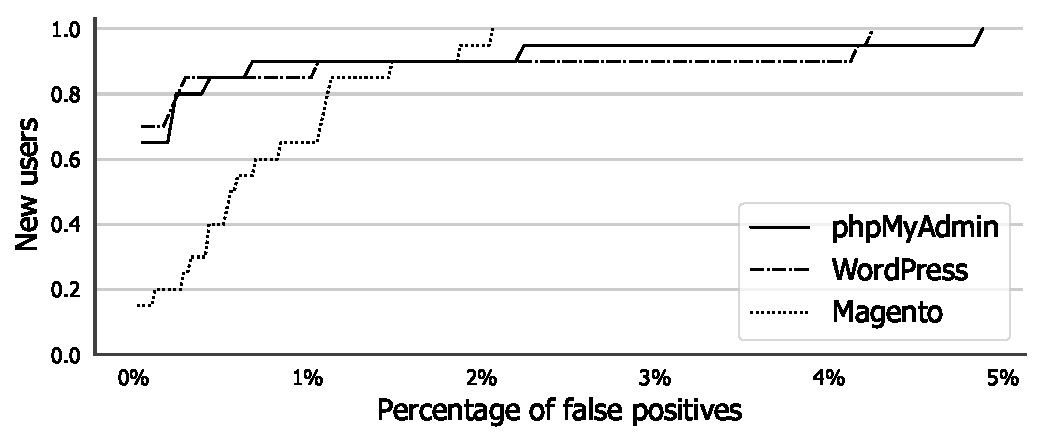
\includegraphics[width=\linewidth]{figures/dbltr/cdf_falsepositives_bw.pdf}
    \caption{CDF of observed false positives from the perspective of new users. The X axis depicts the percentage of false positives (i.e., ratio of the number of missing files compared to total used files by each new user).}
    \label{fig:adding_new_users}
\end{figure}

Figure~\ref{fig:adding_new_users} provides the CDF of false positives (i.e., missing files) when adding new users. 
For phpMyAdmin and WordPress, the majority (60-70\%) of users in the leave-one-out experiment could be added to the ``globally-debloated'' web application without any false positives. 
Likewise, more than 85\% of new users would experience breakage in less than 1\% of the overall files that they interact with. 
For Magento, while most new users assigned to the ``globally-debloated'' web application would experience some breakage, most still fall below the 1\% threshold. 
Overall, across all three web applications in our dataset, even for users with notably unique behavior, we observe less than 5\% of the overall files missing when their usage behavior traces were omitted from the training dataset. 

Looking at the unique behavior of users that led to false positives, in phpMyAdmin, we observe enabling multistep authentication modules, using query explainer features, and creating SQL Views to be the underlying cause (i.e., desired functionality that is unavailable to new users). For WordPress, customizing the RSS feed, using specific text blocks in posts such as text art, and quotes, and using less popular embedding protocols led to false positives under this aggressive user-assignment strategy. Finally, for Magento, various users interacted with unique features.  These features include third-party integrations (e.g., monitoring, marketing, and automation services), PDF invoices, and wish lists. 

Overall, our results show that the modular architecture of \dbltr{} allows it to successfully serve different types of environments. For environments with fixed workloads or where security is prioritized over usability, \dbltr{} can be used to assign new users to a globally-debloated web application. Alternatively, when administrators are unsure about the needs of new users, \dbltr{} can be used to serve the original version of a web application to these users, until enough usage traces are collected to allow \dbltr{} to create new roles and clusters. In either scenario, the security-related debloating benefits of existing users are not in any way compromised when new users are added to a system. In terms of removing users, administrators can merely disable user-role mappings in \dbltr{}'s configurations and optionally delete containers that do not have any roles associated with them.

\subsection{Main Takeaways}

\noindent\textbf{Static roles in web applications are over authorized and administrators only need a subset of the available features:} 
Throughout our user study, we determined that administrators of the same web application use different subsets of the features available to them. 
While in theory, administrators have full access to every feature in the administration panel, in practice only 25\% and 52\% of the lines in the administrative panels of phpMyAdmin and WordPress respectively, were among the commonly exercised features. 
Evidently, the existing authorization mechanisms of these applications aim to offer access to a large variety of features whereas, in reality, administrators only need a subset of them. 
\dbltr{} builds an accurate list of required features and enforces the principle of least privilege via debloating. 

\noindent\textbf{One-size-fits-all debloating still produces bloated web applications:} 
As demonstrated by this work and the literature, debloating web applications is highly effective in reducing the attack-surface of web applications by removing unused features and their underlying vulnerabilities. 

The global debloating approach explored by the prior work produces one debloated web application which as demonstrated by our analysis, can contain as much as 29\% extra LLOC compared to what users actually need. 
In this work, we integrated \dbltr{} with a dynamic debloating scheme and demonstrated that \dbltr{} can provide improvements across all debloating metrics. 
We demonstrated that in the case of global debloating, users in at least half of the roles would be provided with larger web applications containing 5,000-60,000 more lines of code than required, and exposed to 40\%-70\% more CVEs.

% \noindent\textbf{Clustering users with similar behavior together reduces the likelihood of broken features:} 
% In Table~\ref{tab:augmented_coverage} we reported that 15-38\% of files covered by each user in a cluster had new functions covered by other users in the same cluster. 
% Moreover, 29-71\% of third-party packages in a cluster and more than half of internal modules had new files added to the coverage from the perspective of each member of the clusters. 
% Both of these results show that clustering users based on their feature usage can produce debloated applications with shrunk attack-surface, while reducing the likelihood of debloating useful features due to overfitting to the specific usage traces of individual users. 

\noindent\textbf{\dbltr{} provides a content delivery environment for debloated web applications:} 
One of the main contributions of our work is our content delivery pipeline which reduces the need for modifications and customizations to target web applications, while keeping the debloating platform entirely invisible to web application users.

\subsection{Limitations} 

%Our work comes with some limitations that we discuss in this section. 

\noindent\textbf{Debloating statistics: }
As part of our analysis on the security benefits of debloating, we mapped 50 CVEs to the source code of our applications. 
We used recent versions of three popular web applications for our user study and debloating.
By the time they become public, CVEs are either already patched or will be patched soon. 
Therefore, we mapped historic CVEs to the patched functions within the new web applications. 
As a result, our reports on CVE reduction indicate the removal of a feature in a more recent version of web application compared to the original version that included the actual vulnerability. This was a ``necessary evil'' since we could not rely on users perfectly replicating their workloads across multiple versions of the same web applications where the original vulnerabilities resided.

\noindent\textbf{Usage behavior modeling: }
Our debloating reports are based on the code-coverage that we collected during our user study. Using our domain knowledge, we have established that the collected dataset is a representative sample of web-application use in the real world. At the same time, different deployments of web applications may be used differently and therefore be debloated differently. Regardless of the degree of use, \dbltr{} can offer concrete security advantages to any existing or future end-to-end debloating strategy by automatically removing code that is not globally required by all users of a given deployment and clustering users to their appropriately-debloated codebase.

\noindent\textbf{Applications with a public interface: }
As depicted in Figure~\ref{fig:system_architecture}, \dbltr{} routes unauthenticated requests towards a ``public'' profile of the debloated web application. 
This profile includes the code for user authentication as well as any other code required for public unauthenticated users. 

For administrative applications that are behind an authentication wall, producing a public profile is straightforward. 
In the example of phpMyAdmin, we only need to perform successful and failed login attempts to generate the baseline code-coverage and debloat the application to produce the public debloated profile. 
For other applications such as WordPress and Magento, this step is more involved. 
First, we would remove all the files that are only available to the administrators, for the WordPress and Magento, this constitutes of removing administrator directories (e.g., \emph{wp-admin} for WordPress and \emph{module-backend} directory for Magento).
Next, we need to only retain the features and modules that are available to public users. 
Therefore, we need to record the code-coverage of unauthenticated users with benign behavior. 

One of the main benefits of our role-based debloating is the removal of features that are not limited by the authentication and authorization boundaries of web applications. 
If attackers can somehow taint the code-coverage of unauthenticated profiles to include a vulnerable piece of code, they can force the debloating pipeline to retain that code, and exploit it later. This only applies to the potential vulnerabilities in the public interface of the applications. 
A possible solution to this problem is to use artificial modeling techniques, such as automated crawlers, to extract the code-coverage of public users. 

\noindent\textbf{Changes to the source code:} 
In this work, we studied the debloating of web applications at a stable state. 
That is, all the required configurations, updates, and plugins were installed and available at the time of debloating. 
For smaller updates, we need to repeat the debloating to produce new copies of the updated web application while not touching the modified files during the update. 
For major version updates that include drastic changes to the architecture of the source code and modules, we would need to collect the code-coverage traces again. This limitation is shared by all debloating systems that offer security benefits via late-stage code transformations. Note however that \dbltr{} can be used to stage a move from the old version of a web application to the new version by slowly migrating users from their old containerized environments to the new ones, one role at a time.

\noindent\textbf{Number of users of the web applications:} 
In our user study, we hired a total of 60 participants (20 participants for each web application). 
While most websites are operated by a small number of administrators, there clearly exist web applications (such as popular social networks) with billions of users and thousands of administrators. Understanding how \dbltr{} could be used in such an environment requires the collaboration of a large operator, something which we do not have access to. \dbltr{}'s current architecture does allow for horizontal scaling of servers, enabling it to serve an arbitrary number of users and roles. As such, we hope that, through the open-sourcing of our system, large organizations will be able to evaluate \dbltr{} in their environments and user populations.